\question{
  \item Considere a rede da figura, composta por cinco comutadores Ethernet (Bridges):
  $V$, $W$, $X$, $Y$, $Z$, um hub e quatro estações: $A$, $B$, $C$, $D$. Considera-se que o identificador
  de cada comutador é igual ao menor dos endereços MAC das suas interfaces (indicados
  simplificadamente junto a cada ligação) - por exemplo, o identificador do comutador
  $W$ será $10$. Todas as ligações têm custo unitário. As tabelas estão inicialmente vazias.

  \begin{figure}[H]
    \centering
    \includesvg[width=\textwidth]{assets/016.svg}
  \end{figure}

  \textbf{Disclaimer:} resolução da autoria do Pedro Chaparro, retirada \href{https://resumos.leic.pt/rc/ligacao-dados/}{daqui}.
}

\begin{enumerate}[leftmargin=\labelsep]
  \subquestion{
  \item Usando o algoritmo spanning tree classifique as interfaces de cada um dos
        comutadores em raiz, designada, ou bloqueada, e indique as BPDUs enviadas por cada
        comutador em cada uma das suas interfaces quando em regime estacionário.
        }

        Em primeiro lugar, é relevante realçar que o comutador raiz será, claro,
        $V$, pois é o comutador com menor identificador ($5$). Igualmente
        relevante é recordar que o formato das BPDU é o seguinte:

        $$
          (\texttt{Root Bridge ID}, \texttt{Root Path Cost}, \texttt{Bridge ID de quem enviou}, \texttt{Port ID de quem enviou})
        $$

        De seguida, vamos procurar calcular as \textit{root ports} em cada comutador,
        que representam os portos pelo qual se consegue, com menor custo, chegar
        à raiz. Tanto as interfaces vizinhas do comutador como as em que não há empate são triviais,
        estando representadas na figura abaixo:

        \begin{figure}[H]
          \centering
          \includesvg[width=0.5\textwidth]{assets/016ab.svg}
        \end{figure}

        Note-se, contudo, que há cenários em que há empate no custo. Nestes casos,
        escolhe-se a interface com menores valores nos dois outros identificadores
        da BPDU (sendo estes os que têm maior prioridade). Quanto ao que à imagem
        acima diz respeito, só nos resta determinar a root port em $Z$: para tal, examinam-se
        as BPDUs como supra-indicado:

        $$
          X \to Z: (5, 2, 20, 22), \quad
          Y \to Z: (5, 1, 30, 31), \quad
          W \to Z: (5, 1, 10, 12), \quad
          W \to Z: (5, 1, 10, 13)
        $$

        $X$ é descartado por ter um custo maior, $Y$ por ter um identificador de bridge maior,
        e por fim escolhemos o porto $12$ de $W$ por ter um identificador de porto menor.
        Assim sendo, temos atualmente as \textit{root ports} representadas na figura abaixo:

        \begin{figure}[H]
          \centering
          \includesvg[width=0.5\textwidth]{assets/016ac.svg}
        \end{figure}

        De seguida, vamos descobrir as \textit{designated ports}: para segmento de
        rede (as \textit{nuvens} na figura), qual é o caminho mais barato para a raiz?
        A análise é feita de forma em tudo análoga à anterior, analisando as BPDUs,
        e ficamos com as seguintes \textit{designated ports} (note-se que todos os portos
        do comutador raiz são, por definição, \textit{designated ports}, a não ser
        que não estejam ligados a nenhum segmento de rede):

        \begin{figure}[H]
          \centering
          \includesvg[width=0.5\textwidth]{assets/016ae.svg}
        \end{figure}

        Todos os restantes portos ficam bloqueados, pelo que ficamos com a rede
        completamente classificada:

        \begin{figure}[H]
          \centering
          \includesvg[width=0.5\textwidth]{assets/016af.svg}
        \end{figure}

        \subquestion{
  \item Para a sequência de envio de tramas: ($A \to B$, $C \to D$, $C \to A$, $B \to A$, $D \to C$),
        indique as interfaces sobre as quais são transmitidas cópias das tramas respectivas
        e qual o estado das tabelas de expedição de cada comutador no final das várias transmissões.
        }

        Inicialmente, as tabelas em todos os comutadores estão vazias. Vamos procurar preenchê-las,
        com o enviar de cada trama, com pares $(\texttt{host de origem}, \texttt{interface pela qual recebeu})$.
        A tabela abaixo, a par do desenho, mostra precisamente o \textit{flooding} da rede
        aquando do envio de cada trama - note-se a particularidade do hub, que ao
        contrário dos outros comutadores, faz \textit{broadcast} para todos os
        vizinhos, inclusive quem lhe enviou a trama.

        \begin{figure}[!ht]
          \centering
          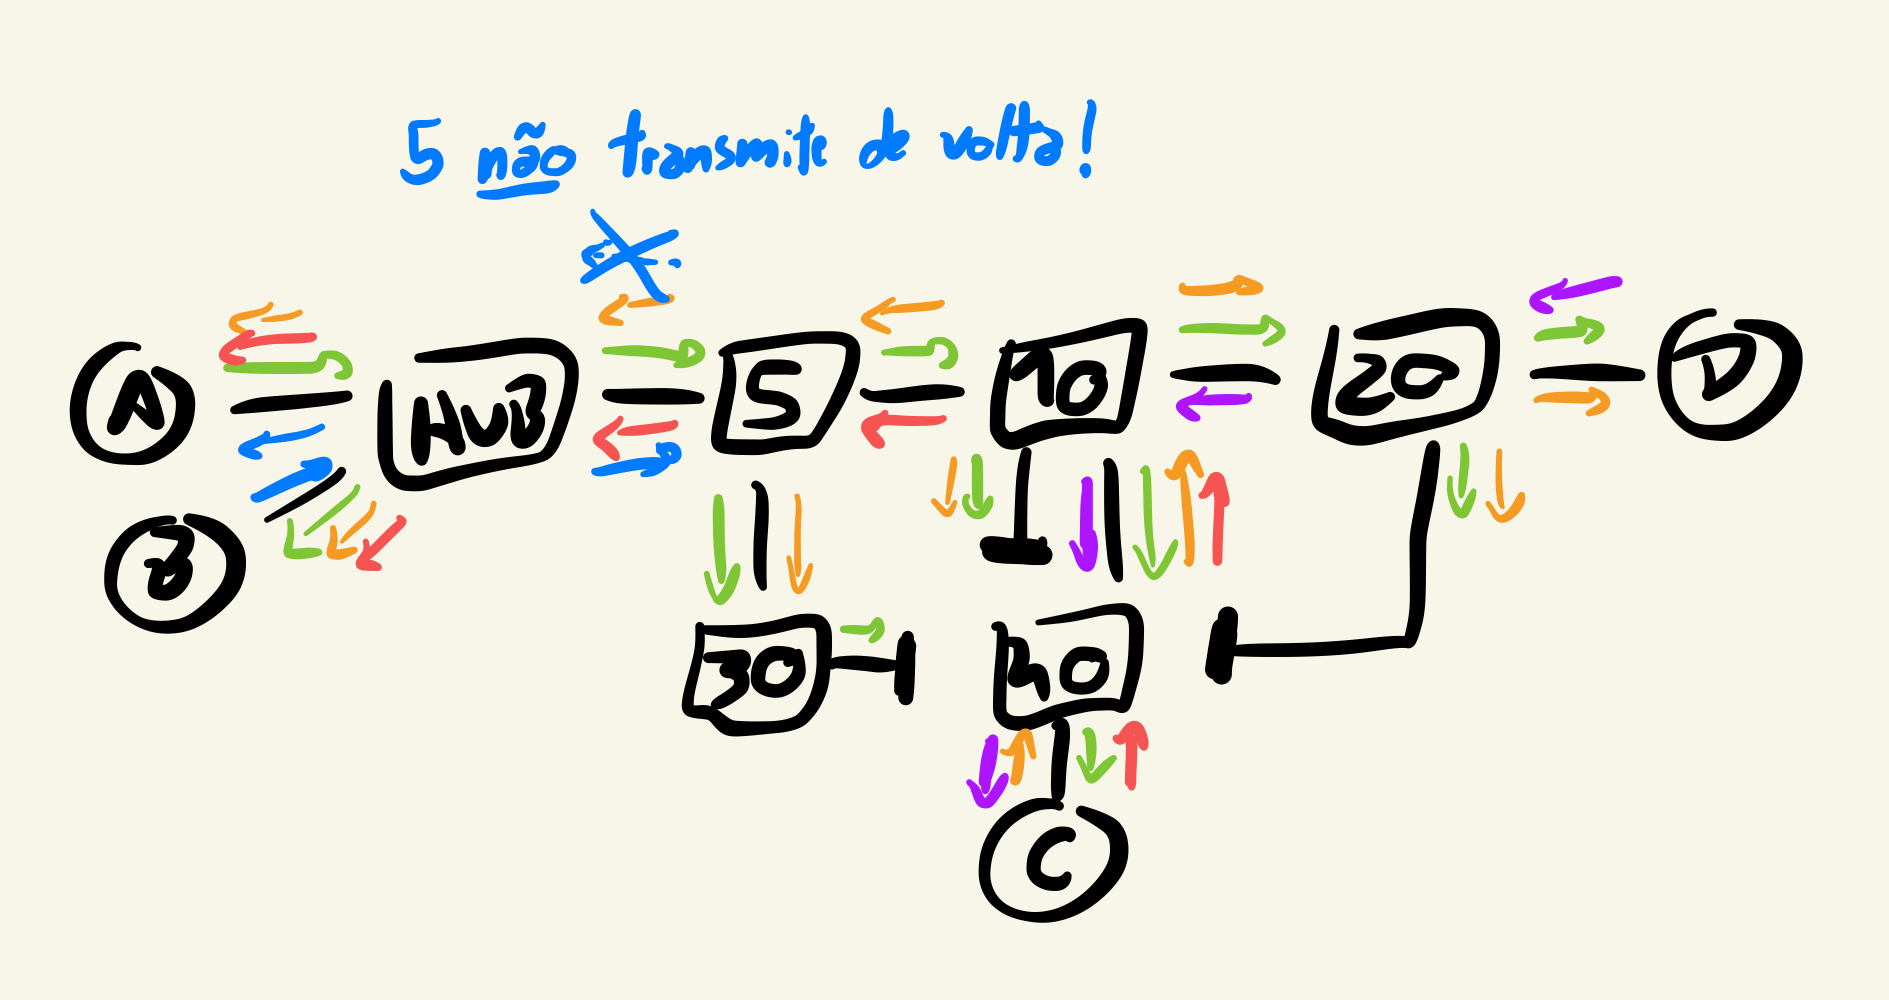
\includegraphics[width=0.45\textwidth]{assets/016b.png}
          \qquad
          \centering
          \begin{tabular}{l|l|l|l|l|l}
                                          & V(5)                     & W(10)                     & X(20)                     & Y(30)                     & Z(40)                     \\ \hline
            \textcolor{green}{A $\to$ B}  & \textcolor{green}{A, 5}  & \textcolor{green}{A, 10}  & \textcolor{green}{A, 20}  & \textcolor{green}{A, 30}  & \textcolor{green}{A, 42}  \\
            \textcolor{orange}{C $\to$ D} & \textcolor{orange}{C, 6} & \textcolor{orange}{C, 12} & \textcolor{orange}{C, 20} & \textcolor{orange}{C, 30} & \textcolor{orange}{C, 44} \\
            \textcolor{red}{C $\to$ A}    & \textcolor{red}{C, 6}    & \textcolor{red}{C, 12}    & -                         & -                         & \textcolor{red}{C, 44}    \\
            \textcolor{blue}{B $\to$ A}   & \textcolor{blue}{B, 5}   & -                         & -                         & -                         & -                         \\
            \textcolor{purple}{D $\to$ C} & -                        & \textcolor{purple}{D, 11} & \textcolor{purple}{D, 21} & -                         & \textcolor{purple}{D, 42}
          \end{tabular}
        \end{figure}
\end{enumerate}